% !TEX root = ../main.tex
\subsubsection{Offline Reconstruction}
\label{11.230::offline_reconstruction}
% --+ CLARA +-------------------------------------------------------------------
    The CLAS12 reconstruction and analysis process is facilitated by a data-stream processing framework called CLARA.
    CLARA adopts a service-oriented architecture, allowing the construction of software applications using micro-services that are connected via data-stream pipes \cite{gyurgyan2016}.

    In this framework, each service plays a specific role.
    It receives input data, processes it according to its functionality, and produces output data.
    The input and output data are organised in tabular structures known as ``banks'', which are configured by the service developer to match the specific requirements of the service.

    The services within CLARA form a data-flow path, where the output of one service becomes the input for the next service in the sequence.
    This design enables a flexible and versatile data processing application, as each service can be individually improved or replaced without necessitating structural changes to the framework.

    To ensure consistency and modularity, the CLAS12 services are extensions of an abstract reconstruction engine.
    This engine provides common components such as initialisation and event processing methods, reducing the development complexity of individual micro-services and enforcing a uniform structure throughout the framework.

    By leveraging the CLARA framework, the CLAS12 experiment benefits from a modular and adaptable data processing pipeline, allowing for efficient reconstruction and analysis of the collected data.
    The service-oriented architecture and data-stream processing approach contribute to the flexibility, scalability, and maintainability of the CLAS12 software framework.

    \begin{figure}[b!]
        \centering\frame{
        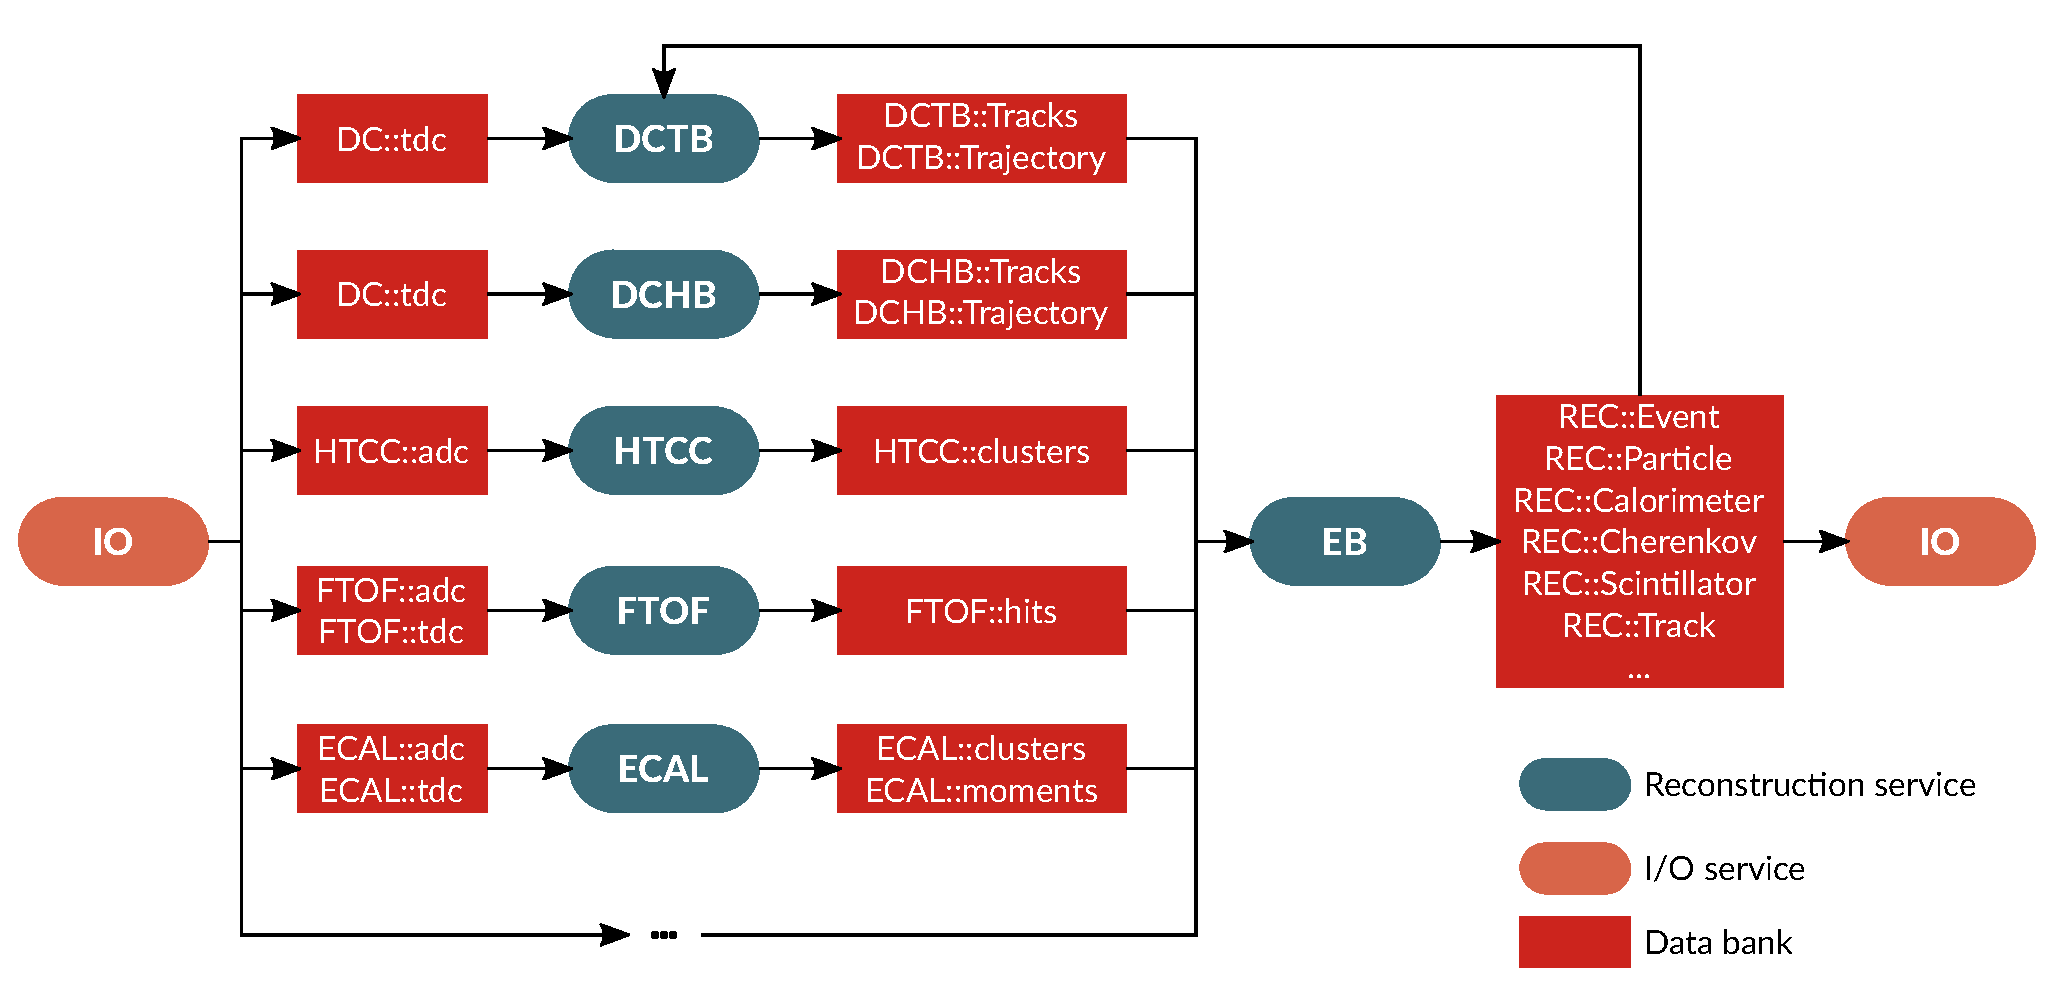
\includegraphics[width=\textwidth]{230recon_chain.pdf}}
        \caption[CLAS12 Reconstruction Chain.]{Graphical representation of the CLAS12 interdependencies between services and banks.
        The I/O service reads events from the input file and distributes them to the reconstruction services chain for processing.
        Each service reads the relevant banks, applies the reconstruction algorithm, and provides output banks that are passed to the next service in the chain.
        The Event Builder (EB) service is executed as last in the chain; it collects the relevant banks from all CLAS12 subsystems services and produces event, particle, and detector response banks that are written to the output file.
        Source: Own elaboration, using \href{https://inkscape.org/}{Inkscape}.}
        \label{fig::11.230::recon_chain}
    \end{figure}

% --+ CLAS12 reconstruction +---------------------------------------------------
    The CLAS12 data reconstruction process involves data reader services that access decoded detector data stored in banks.
    Each entry in the bank represents a decoded detector hit and contains information such as sector, layer, component, order, and digitised data like signal charge, amplitude, time, or pedestal.

    During the decoding stage, similar bank structures are created for various quantities required for event reconstruction, including hits, clusters, and tracks.
    Reconstruction algorithms specific to each CLAS12 subsystem fill these banks.
    The data persistence service appends and writes these banks to a file for later analysis.

    The reconstruction algorithms are implemented as services that operate on input banks and produce output banks, which are then passed to subsequent algorithms in the reconstruction chain.
    The order in which the services are chained reflects the overall sequence of CLAS12 event reconstruction and the dependencies between subsystems.

    The first step is the reconstruction of charged particle tracks in the Central and Forward Detector tracking systems, based on the recorded hit positions in the respective detectors.
    This process is known as ``hit-based'' tracking.

    Simultaneously, hits recorded in other detectors are processed to reconstruct the energy and time of the associated particle interactions.
    The Event Builder (EB) service matches these reconstructed quantities with the tracks based on position and time information.
    Hits that are not matched to any track are retained as neutral particle candidates.
    The EB also determines the event ``start time'' and identifies the reconstructed particles.

    Once the event start time is determined, a second iteration of forward tracking, known as ``time-based'' tracking, can be performed.
    This iteration incorporates the drift times in the Drift Chambers, providing improved tracking precision \cite{ziegler2020}.

    An overview of the composition of reconstruction application services, depicting the dependencies between the services, can be found in Figure \ref{fig::11.230::recon_chain}.

    % !TEX root = ../main.tex
\paragraph{Tracking}
% --+ Introduction +------------------------------------------------------------
    \begin{wrapfigure}{r}{0.50\textwidth}
        \centering\frame{
        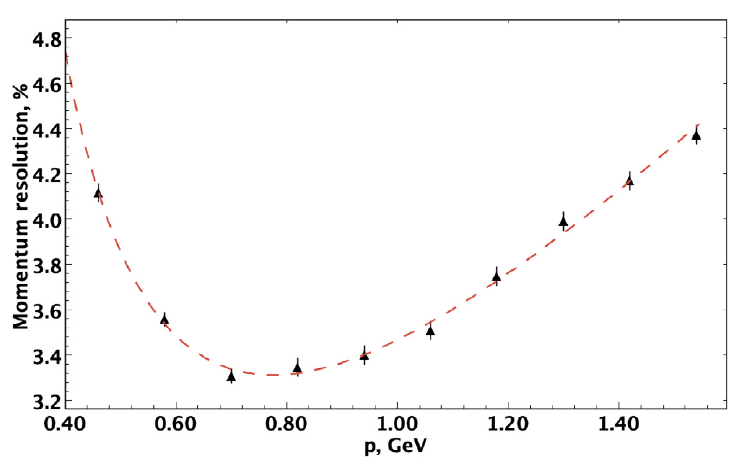
\includegraphics[width=\linewidth]{231cvt_pres.png}}
        \caption[CVT momentum resolution vs. momentum.]{Momentum resolution vs. momentum of simulated protons in the CVT without background.
        Source: \cite{ziegler2020}.}
        \label{fig::11.231::cvt_p_resolution}
    \end{wrapfigure}

    In the CLAS12 event reconstruction, charged particle tracking plays a crucial role and is divided into two main regions: the forward region and the central region.

    In the forward region, charged particles are bent either inward or outward from the beamline by the torus magnet, depending on their charge.
    The magnetic field strength varies along the bending path, with an integral magnetic field ($\int Bdl$) ranging from $2 \text{Tm}$ at $5\degree$ to $0.5 \text{Tm}$ at $40\degree$.
    The forward tracking system responsible for tracking in this region consists of two components: the Forward MicroMegas Tracker (FMT) and the Drift Chambers (DC).

    In the central region, charged tracks are curved into helices by the strong $5 \text{T}$ solenoidal magnetic field.
    The central tracking system comprises the Silicon Vertex Tracker (SVT) and the Barrel MicroMegas Tracker (BMT), which together form the Central Vertex Tracker (CVT).

    These tracking systems in both the forward and central regions use sophisticated detectors to measure the position of charged particle hits, allowing for the reconstruction of particle trajectories.
    By combining information from these detectors and utilising the magnetic field information, the tracking algorithms reconstruct the paths of charged particles, enabling precise determination of their momenta and vertices.

% --+ Reconstruction +----------------------------------------------------------
    In both the forward and central tracking systems, track reconstruction involves two main steps: pattern recognition and track fitting.
    The first step is to identify hits, which are the recorded signals corresponding to a particle passing through a specific detector component.
    These hits are transformed from electronic signals into the position of the track within the geometry of the detector subsystem.

    \begin{wrapfigure}{r}{0.50\textwidth}
        \centering\frame{
        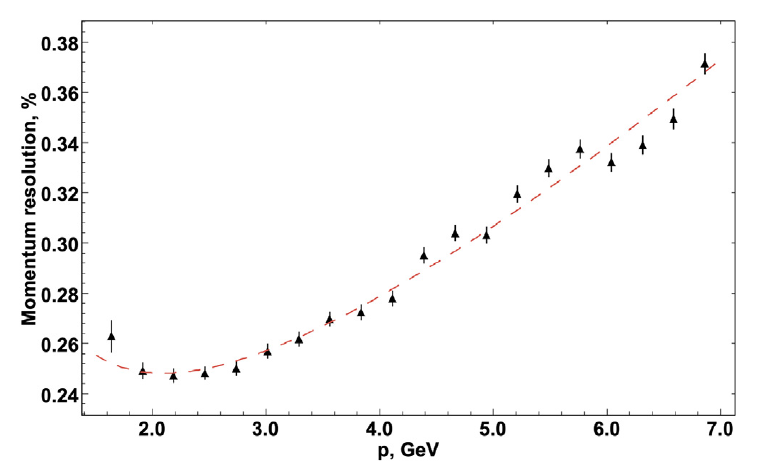
\includegraphics[width=\linewidth]{231dc_pres.png}}
        \caption[DC momentum resolution vs momentum.]{Momentum resolution vs. momentum in the DC evaluated using pions simulated at $\theta = 15\degree \pm 5\degree$ and at $\phi = 0 \pm 5\degree$ without background.
        Source: \cite{ziegler2020}.}
        \label{fig::11.231::dc_p_resolution}
    \end{wrapfigure}

    A hit is defined as a geometric object that represents a detector element.
    For example, in the central tracker, a hit can be represented by a line corresponding to a strip in the detector.
    These hit objects serve as the input for the pattern recognition algorithms.

    \begin{figure}[t]
        \centering\frame{
        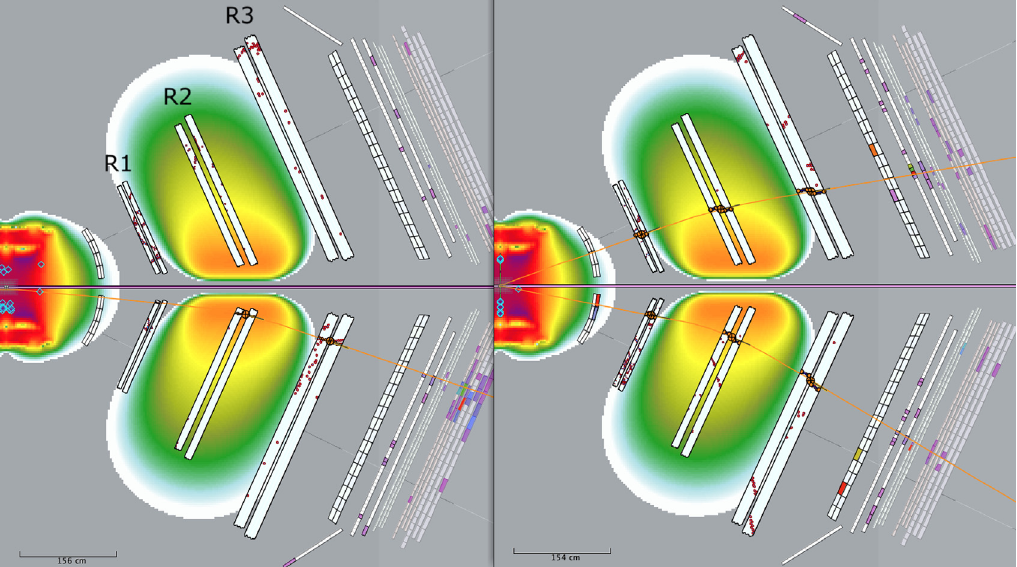
\includegraphics[width=\textwidth]{231ced_event.png}}
        \caption[Particle going through DC.]{Views from CLAS12 Event Display (ced) of charged particle tracks in the DC showing cut-views to highlight different pairs of sectors of the CLAS12 Forward Detector.
        The coloured detector elements are the registered hits and the orange lines are the result of track reconstruction using the hits in the DC.
        The coloured areas about the detectors represent the regions of magnetic field from the torus and the solenoid.
        In these views the beam is incident from the left and the target is located in the middle of the solenoid (at the left edge of the image).
        Source: CED render.}
        \label{fig::ced_event}
    \end{figure}
    Pattern recognition involves identifying clusters of hits and determining the spatial coordinates and corresponding uncertainties for the hits and clusters.
    During the pattern recognition stage, hits that are consistent with belonging to a trajectory, such as a particle track, are identified.
    This set of hits is then fitted to the expected trajectory, considering their uncertainties and incorporating knowledge of the detector material and the detailed magnetic field map.
    Figure \ref{fig::ced_event} illustrates a particle passing through the DC.

% --+ Performance +-------------------------------------------------------------
    The momentum resolutions in the central and forward trackers, as a function of momentum, are shown in Figures \ref{fig::11.231::cvt_p_resolution} and \ref{fig::11.231::dc_p_resolution}, respectively.
    The distributions are fitted with a function of the form $\sqrt{a + bx^2 + c/(1 + d/x^2)}$.
    In both distributions, the degradation of resolution at low momentum is attributed to multiple scattering effects.
    Furthermore, the resolution deteriorates as momentum increases beyond a minimum, primarily because of poorer track curvature resolution.

    For central tracking, a simulated proton sample with momenta ranging from $0.5$ to $2.5 \text{ GeV}$ yields an average CVT reconstruction efficiency of $87.3\%$.
    A slight decrease in efficiency is observed for tracks with momenta below $600 \text{ MeV}$.
    The increased curvature of low transverse momentum ($\text{p}_\perp$) tracks leads to a rise in inefficiency due to acceptance effects.
    The primary source of inefficiency stems from the gaps between the sensitive volumes of the BMT and SVT detectors.

    Regarding forward tracking, the momentum resolution in the DC is evaluated using tracks simulated at $\theta = 15\degree \pm 5\degree$ and $\phi = 0 \pm 5\degree$.
    This range ensures that the majority of tracks fall within the sensitive volume.
    Moreover, the DC momentum resolution exhibits correlation with the polar angle since track curvature is determined by the magnetic field intensity, which is higher at lower angles in the torus field.
    These resolutions are obtained from a Monte Carlo sample that excludes out-of-time backgrounds or misalignments of the tracking volumes \cite{ziegler2020}.

    % !TEX root = ../main.tex
\paragraph{Particle Identification}
% --+ PDG PID +-----------------------------------------------------------------
    The Particle Identification (PID) numbering scheme described here was initially introduced by the Particle Data Group (PDG) in 1988 \cite{yost1988}.
    Its purpose is to facilitate communication and data exchange between different generators, simulators, and analysis packages employed in particle physics.
    The system underwent subsequent revisions and adaptations in 1998 to allow for the systematic inclusion of undiscovered and hypothetical particles \cite{particle1998}.
    The PID convention utilised in this thesis is based on the most up-to-date version available at the time of writing, as referenced from the 2020 Review of Particle Physics by the PDG \cite{particle2020}.

% --+ The Event Builder +-------------------------------------------------------
    The EB is a crucial component within the reconstruction chain, serving multiple functions:
    \begin{itemize}
        \item
            It gathers information from upstream services.
        \item
            It correlates information from sub-detectors to form particles.
        \item
            It implements a general particle identification scheme.
        \item
            It organises the resulting information into a standardised and persistent data bank structure.
    \end{itemize}

    The EB service is executed twice using identical algorithms, first employing hit-based tracks and subsequently using time-based tracks.
    As mentioned previously, the results obtained from the hit-based EB are utilised to initialise time-based tracking.

% --+ Forming particles +-------------------------------------------------------
    In the definition of a reconstructed charged particle within CLAS12, the EB assumes that each reconstructed track in both the FD and the CD will be assigned an identification.
    The corresponding responses from the calorimeter, scintillator, and Cherenkov detectors are then associated with that particle based on geometric coincidences between the detector responses and the track.
    Matching criteria are established, which correspond to the resolution of each specific detector.
    The geometric matching process relies on the Distance of Closest Approach (DOCA) between the track and the detector response.

    A similar procedure is employed for the creation of neutral particles, with the distinction that the seeding is presently performed using unassociated responses from the ECAL for the FD and the CND (or the BAND) for the CD, instead of using tracks.

% --+ Event start time +--------------------------------------------------------
    A start time is assigned to the entire event and serves as the precise reference time for all time-based particle identification procedures.
    The determination of the start time relies on the optimal charged particle candidate in the FD with an associated timing response from the FTOF detector.

    The EB assigns the start time based on the highest energy electron detected in the ECAL.
    If no electron is found in the ECAL, the EB then searches for a positron in the ECAL.
    In the absence of any lepton candidates, the next track in the priority list is a forward-going positive track, which is assumed to be a positive pion ($\pi^+$).
    Finally, if no forward-going positive track is identified, the EB searches for a forward-going negative track, assumed to be a negative pion ($\pi^-$).
    When searching for $\pi^+$ or $\pi^-$ tracks, only the candidate with the highest momentum within each group is considered.

    A parallel event start time is determined from the FT system to facilitate physics analyses and triggers specifically for events where the primary scattered electron is at very forward angles within the FT.

    In such cases, all combinations of charged particles in both the FT and the FD are taken into account.
    The particle in the FT is assumed to be an electron, while all possible hadron mass hypotheses are considered for the FD tracks.
    The combination that exhibits the best time coincidence is selected, and the timing of the resulting FT electron is used to assign the start time.

    A correction to the start time is subsequently applied using the RF signal from the accelerator, in conjunction with the reconstructed event vertex position.
    This correction effectively aligns the event start time with the most accurate measurement of the beam-bunch arrival time at the target.

    The uncorrected measured vertex time of a particle, denoted as $t_v$, can be expressed as follows
    \begin{equation*}
        t_v = t - \frac{P_L}{\beta c},
    \end{equation*}

    Here, $t$ represents the measured time response (e.g., in a scintillator), $P_L$ is the path length between the primary interaction vertex and the corresponding response, and $\beta c$ denotes the speed of the particle.

    Next, we calculate the time difference $\Delta t_{RF}$ between $t_v$ and the nearest beam bunch using the following formula
    \begin{equation*}
        \Delta t_{RF} = t_v + \frac{z_0 - z_v}{c} - t_{RF} - \frac{N}{2f_{RF}},
    \end{equation*}

    In this equation, $z_v$ represents the $z$-coordinate of the event vertex position, $z_0$ is the reference position calibration at the center of the target, and $c$ denotes the speed of light in vacuum.
    $t_{RF}$ and $f_{RF}$ correspond to the measured and calibrated RF time and frequency of the accelerator.
    These values can either be $2.004 \text{ ns}$ and $249.5 \text{ MHz}$, or $4.008 \text{ ns}$ and $499 \text{ MHz}$, respectively.
    During the reconstruction process, these values are obtained from the Run Conditions Database.

    \begin{wrapfigure}{r}{0.49\textwidth}
        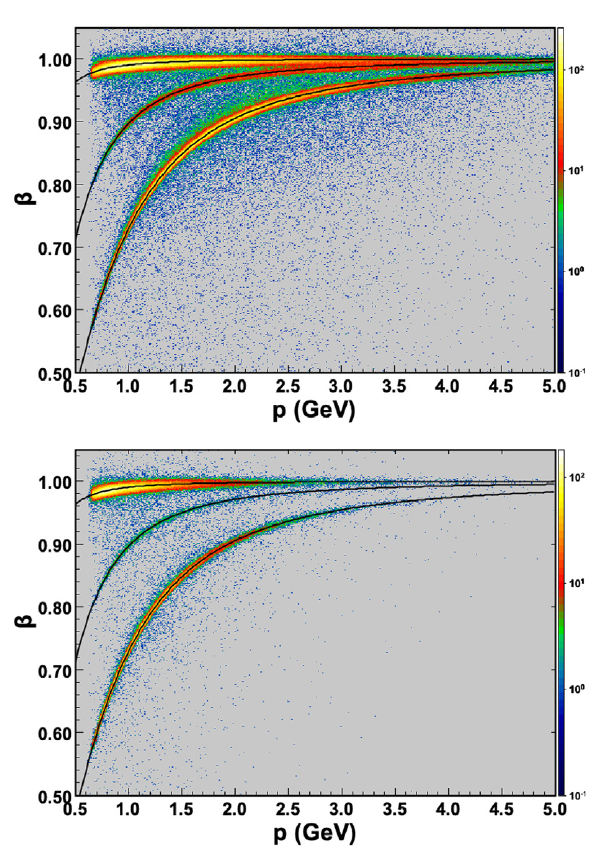
\includegraphics[width=\linewidth]{232pos_pid.png}
        \caption[Particle $\beta$ vs. momentum for positively charged tracks]
        {Particle $\beta$ vs. momentum from simulation data for positively charged tracks with their start time from an electron in the FD (top plot) or in the FT (bottom plot).}
        \floatfoot{Source: \cite{ziegler2020}.}
        \label{fig::11.232::positive_pid}
    \end{wrapfigure}

    Subsequently, the time can be further corrected to the nearest beam bunch using the equation
    \begin{equation*}
        \Delta t^\prime_{RF} = \text{mod}\left(\Delta t_{RF}, \frac{1}{f_{RF}}\right) - \frac{1}{2f_{RF}},
    \end{equation*}

    This correction allows for RF-correction to $t_v$. Thus, we obtain a final RF- and vertex-corrected start time for the event, defined as
    \begin{equation*}
        t' = t_v - \Delta t^\prime_{RF}.
    \end{equation*}

% --+ Charged particle identification +-----------------------------------------
    The subsequent step involves a basic particle identification scheme designed to be flexible enough to accommodate various physics analyses while retaining essential information for future refinement of the criteria.

    For charged particles, the identification process begins by utilising calorimetry and Cherenkov information to positively identify $e^-/e^+$ candidates in the FD.
    If the measured energy deposition aligns with the expected sampling fraction of the ECAL and the photoelectron response from the HTCC aligns with $\beta \sim 1$, the particle is assigned as an $e^-$ or $e^+$ based on the sign of curvature determined from forward tracking with the DC in the presence of the torus magnetic field.

    The remaining charged particles are then assumed to be hadrons and are assigned an identity solely based on timing information.
    The $p, K, \pi$ candidate with the smallest time residual is selected.
    This time residual is calculated as the difference between the measured flight time of the particle and the flight time computed for a specific mass hypothesis.

    Figure \ref{fig::11.232::positive_pid} presents the $\beta$ vs. momentum distributions for forward-going positively charged hadrons reconstructed using data from the FTOF and DC subsystems.
    The electron is reconstructed either in the FD (top) or in the FT (bottom).
    The computed curves for different mass hypotheses are superimposed on the distributions.

    \begin{wrapfigure}{r}{0.50\textwidth}
        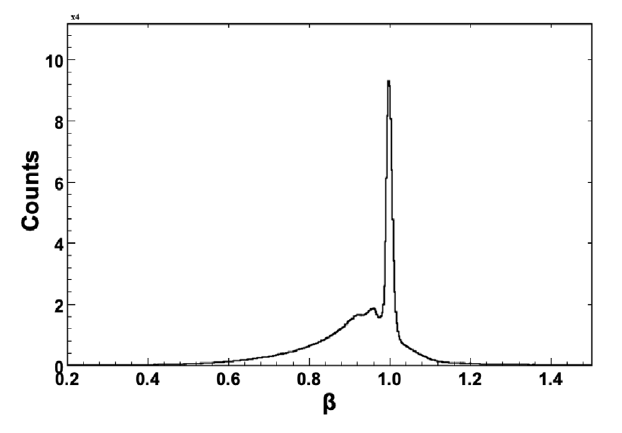
\includegraphics[width=\linewidth]{232n_gamma.png}
        \caption[$\beta$ distribution of neutrals]
        {$\beta$ distribution for neutral particles as measured by the ECAL from simulation data, showing a sharp peak at $\beta = 1$ from photons and a broader, slower distribution from neutrons.}
        \floatfoot{Source: \cite{ziegler2020}.}
        \label{fig::11.232::neutrons_and_gamma}
    \end{wrapfigure}

% --+ Neutral particle identification +-----------------------------------------
    To identify neutral particles, the analysis assumes the presence of only neutrons and photons, distinguished solely by timing and topological information.
    In the FD, the identification is based on the ECAL, while in the CD, it relies on the CND.
    The reconstructed cluster positions of these detectors are used to calculate the particle's travel path from the event vertex, assuming a straight-line trajectory.

    If the measured $\beta$ value is close to $1$, the particle is identified as a photon; otherwise, it is identified as a neutron.
    For photons in the FD, the momentum is determined from the deposited energy and the ECAL sampling fraction \cite{asryan2020}.
    For neutrons, the momentum is assigned based on the measured $\beta$, assuming the mass of a neutron.

    Figure \ref{fig::11.232::neutrons_and_gamma} illustrates an example of the reconstructed $\beta$ values for neutral particles in the FD, demonstrating the separation between photons and neutrons.

% --+ Particle identification performance +-------------------------------------
    A particle identification quality factor, represented as a signed-$\chi^2$ or pull, is assigned based on the contributions from individual detector subsystem responses and their resolutions.
    For $e^-/e^+$ identification, the resolution-normalised distance from the expected ECAL sampling fraction is utilised, while for charged hadrons, the resolution-normalised time difference is employed.
    The resulting information is organised into standardised output bank structures for physics analysis.
    This includes the particle four-vectors, associated detector responses, and global event information such as beam RF and helicity details.

    The accuracy of the currently implemented particle identification algorithm can be estimated by comparing the assigned particle identification with the true identification in Monte Carlo simulations.
    Table \ref{tab::11.232::reconstruction_pid} presents the particle identification matrix for the FD (left) and CD (right).
    The values are derived from simulations involving electron-hadron or electron-photon pairs with hadron and photon momenta ranging from $1$ to $2.5 \text{ GeV}$ and electron momenta ranging from $1$ to $9 \text{ GeV}$.
    The diagonal elements represent cases where the particle is correctly identified, while the off-diagonal elements represent cases of misidentification \cite{ziegler2020}.

    \begin{table}
        \begin{tabularx}{\textwidth}{XXXXXXXXXXXXX}
            \multicolumn{7}{c}{\textit{Forward Detector Truth}} & & \multicolumn{5}{c}{\textit{Central Detector Truth}}  \\
            \cmidrule{1-7} \cmidrule{9-13}
                     & $e$      & $\pi$ & $K$  & $p$  & $n$  & $\gamma$ & &       & $\pi$    & $K$  & $p$  & $n$  \\
            \cmidrule{1-7} \cmidrule{9-13}
            $e$      & 0.98     &       &      &      &      &          & & $\pi$ & 0.84     & 0.14 & 0.00 &      \\
            $\pi$    &          & 0.93  & 0.10 & 0.00 &      &          & & $K$   & 0.11     & 0.80 & 0.01 &      \\
            $K$      &          & 0.03  & 0.80 & 0.00 &      &          & & $p$   & 0.03     & 0.04 & 0.95 &      \\
            $p$      &          & 0.03  & 0.02 & 0.98 &      &          & & $n$   &          &      &      & 0.11 \\
            \cmidrule{9-13}
            $n$      &          &       &      &      & 0.66 & 0.01     & &       &          &      &      &      \\
            $\gamma$ &          &       &      &      & 0.14 & 0.95     & &       &          &      &      &      \\
            \cmidrule{1-7}
        \end{tabularx}

        \caption[Particle identification matrix]
        {Particle identification matrix for the FD (left matrix) and CD (right matrix).
        The FD matrix is based on simulated hadrons and photons with momentum between $1$ and $2.5 \text{ GeV}$, and electrons up to $9 \text{ GeV}$.
        The CD matrix is based on simulated hadrons with momentum between $0.3$ and $1.1 \text{ GeV}$.
        The diagonal elements are correctly identified, while the off-diagonal elements are misidentified.
        Detector inefficiencies are included.}
        \label{tab::11.232::reconstruction_pid}
    \end{table}

